\chapter{Escalamiento}

Scrum es aconsejable para ser óptimo en equipos chicos y proyectos pequeños, con agrupación de personas de múltiples disciplinas en un solo equipo para maximizar el ancho de banda de las comunicaciones, la visibilidad y la confianza. Esto sucede porque cuando los equipos son grandes aumenta el acoplamiento de individuos complejizando las comunicaciones y dificultando la coordinación y el buen desarrollo de las reuniones Scrum. Además se desprende del principio o Ley de Brooks, que dice que cuando se agregan personas a un proyecto o equipo aumentan los canales de comunicación pudiendo generar sobrecarga de comunicación. Por este motivo y desde un punto de vista purista, cuando se quiere implementar Scrum en proyectos grandes que requieren muchas personas, en su forma ortodoxa, no es recomendable. Pero se han encontrado maneras organizativas para aplicar Scrum en estos casos, como así también en grandes organizaciones. A esto se llama "Scaling Scrum" o Escalamiento de Scrum.

En "Scaling Scrum" los desafíos más importantes son: manejar las dependencias e integrar el trabajo en todos los niveles. En general Scrum se escala mediante reproducción de equipos con configuraciones adecuadas y la cohesión y acoplamiento mediante algún sistema de integración ágil, como el uso de "Scrum de Scrum", equipos de Product Owners, equipo de integración, etcétera. Hay varios casos que se pueden investigar, como por ejemplo las implementaciones de: Google, Spotify, Adobe, Nexus, etc.

\section{Equipos}

En "Scaling Scrum" los equipos funcionan como células que, a medida que la organización se expande, se clonan sus estructuras como en reproducción celular. La estructura de las células depende del problema que se quiere resolver. Un equipo puede ser un Scrum-Team formado por diferentes roles, tales como: UX, SM, PO, BA, QA, FE Dev, BE Dev, etcétera. Por ejemplo, un equipo puede estar formado por: PO, SM, UX, 3 FE Dev y 3 BE Dev; otra estructura puede ser: PO, SM, BA, QA, 2 FE Dev y 2 BE Dev. En esta vía tenemos tres lineamientos básicos de configuración: equipos Scrum de características, equipos Scrum de componentes y uno mixto. Y cada una de estas modalidades pueden tener diversas configuraciones de roles.


\subsection{Equipos de características}

Abordar el problema de proyectos grandes con "Equipos Scrum de características" consiste en la conformación de equipos totalmente multi-funcionales con un enfoque "Whole Team"\footnote{En un enfoque Whole Team todos pueden hacer, hasta cierta medida, alguna tarea de otro\cite{Juan-Gabardini-2015}.} con características de miembros full-stack, capaces de operar en todos los niveles de la arquitectura del producto con el fin de ofrecer las características centradas en el cliente (ver figura \ref{fig:ScrumTeamsByFeatures}). O sea que cada equipo trabaja sobre determinadas características de producto (Features) o PBIs desarrollando todos los niveles del sistema a desarrollar (end-to-end). En este sentidos, los equipos son homogéneos entre sí pero heterogéneos internamente, con integrantes de habilidades diversas y características profesionales multidisciplinares. Para lograr esto se debe conformar una organización de aprendizaje donde los equipos practican el aprendizaje continuo, donde aprenden para abarcar los componentes arquitectónicos.

\begin{figure}[h]
  \centering
  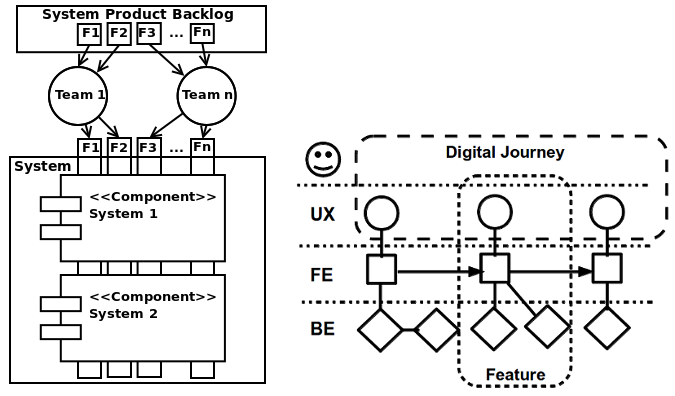
\includegraphics[width=0.80\textwidth]{ScrumTeamsByFeatures}
  \caption{Esquema de equipos de características}
  \centering
  \label{fig:ScrumTeamsByFeatures} %\ref{fig:ScrumTeamsByFeatures}
\end{figure}

En esta arquitectura de organización es necesario coordinar el trabajo de los diferentes equipos. Los Scrum Master deben reunirse con regularidad, promoviendo la transformación a través de una lista visible de los impedimentos de organización. Los Scrum Master, además deberán estar familiarizados con biografía relacionada a este problema de escalabilidad como "Scaling Lean and Agile Development" \cite{Larman-Vodde-2008}.

\subsection{Equipos de componentes}

Abordar el problema de proyectos grandes con "Equipos Scrum de componentes" (ver figura \ref{fig:ScrumTeamsByComponent}) consiste en que cada equipo sólo es responsable de la ejecución de ciertos componentes dedicados en el sistema de los cuales el equipo es dueño de su desarrollo. Desde esta perspectiva se pueden tener equipos dedicados por capas (capa front-end, capa de servicios, capa de persistencia) y por componentes de arquitectura de software (diferentes componentes como librerías, servicios o subsistemas).

\begin{figure}[h]
  \centering
  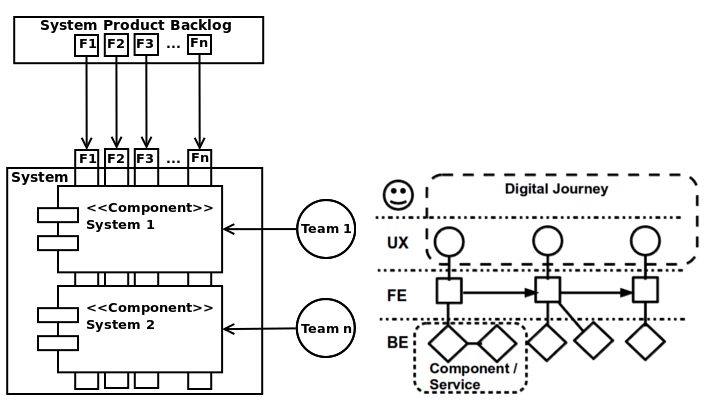
\includegraphics[width=0.80\textwidth]{ScrumTeamsByComponent}
  \caption{Esquema de equipos de componentes}
  \centering
  \label{fig:ScrumTeamsByComponent} %\ref{fig:ScrumTeamsByComponent}
\end{figure}

Para terminar una PBI o historia de usuario hay en la mayoría de los casos la necesidad de dividir las historias en partes más pequeñas que podrían ser implementadas dentro de un solo componente. Además se genera dependencias entre los diferentes equipos haciendo necesario procesos de integración periódica y coordinación de equipos. En muchos casos, una sola historia de usuario no se puede implementar dentro de un único sprint y, en su defecto, depende de los resultados de otras historias desarrolladas por otro equipo que aún no están disponibles. A esto se lo llama "pipeline" y debe evitarse en lo posible o gestionarse apropiadamente.

La ventaja de utilizar equipos de componentes es que es más fácil asegurar una determinada arquitectura del sistema. Por ejemplo si se quiere asegurar una Arquitectura SOA o una de Microservicios que está orientada a componentes. Esta idea está, entre otras cosas, basada en la "Ley de Conway"\footnote{Conway's Law \cite{Conway-1968} no es exactamente una ley, sino que es más bien una observación que Conway publicó en 1968.} que sugiere que las organizaciones pueden replicar su arquitectura en los productos que ellas producen \cite{Martin-Fowler-2014}. 

Por otro lado, puede tener como desventaja que las personas se pueden especializar sólo en pequeñas partes del sistema y el conocimiento global sobre el sistema en su conjunto podría perderse \cite{Scrum-Institute-2015}. En este caso podría tener lugar una optimización local, ya que el equipo a veces puede tomar decisiones que están optimizadas para el componente individual, pero las mejores soluciones desde una perspectiva del sistema total podrían haber sido desestimadas u obviadas.


\subsection{Equipos mixtos}

También es posible la configuración de equipos mixtos que son la combinación de equipos de características y de componentes (ver figura \ref{fig:ScrumTeamsMix}).

\begin{figure}[h]
  \centering
  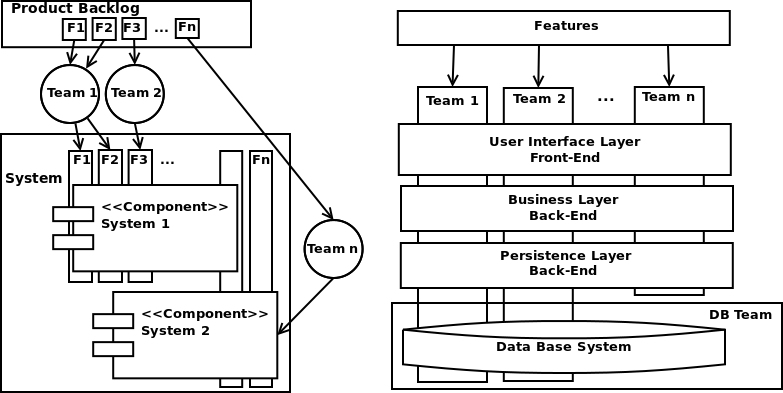
\includegraphics[width=0.99\textwidth]{ScrumTeamsMix}
  \caption{Ejemplo de equipos mixtos.}
  \centering
  \label{fig:ScrumTeamsMix} %\ref{fig:ScrumTeamsMix}
\end{figure}

\section{Integración}

\subsection{Scrum de Scrum}

Scrum de Scrum es una forma de organización y técnica para escalar Scrum a grupos grandes de personas u organizaciones con proyectos grandes, programas o portfolios. Consiste en distinguir un integrante con el rol de Embajador, denominado "Ambassador", por cada Equipo Scrum \cite{Stefanini-2013}. El Embajador será quien participará en reuniones Daily con Embajadores de otros equipos. A esta reunión de Embajadores se la llama "Scrum de Scrum" o SoS. Habitualmente se usa que el rol de Embajador lo desempeñe el Scrum Master, pero puede ser desempeñado por otro integrante del Equipo de Desarrollo. También puede ser desempeñado por un integrante del Equipo acompañado del Scrum Master.

La reunión SoS se comporta como una Daily donde los Embajadores reportan la situación de su equipo y sus impedimentos. El embajador de cada equipo comenta la respuesta a las siguientes tres preguntas:

\begin{itemize}
\item \textbf{¿Qué hicimos ayer?}
\item \textbf{¿Qué vamos a hacer hoy?}
\item \textbf{Si tenemos obstáculos: ¿Qué impedimentos tenemos?} ¿Qué impedimentos tenemos a nivel de equipo? ¿Si algún otro equipo nos bloquea para algo? ¿Si bloqueamos en algo a algún otro equipo?
\end{itemize}

La SoS puede ser facilitada y moderada por una persona que puede desempeñar un rol de facilitador, coordinador e integrador inter-equipos. Este rol puede tener diferentes nombres y el SBOK lo denomina Chief Scrum Master o CSM. El CSM apoyará y brindará soporte a los SM de diferentes equipos.

\subsection{Scrum de Scrum de Scrum}

En organizaciones donde hay muchos Equipo Scrums trabajando en varias partes de un proyecto o producto grande, puede ser necesario otro nivel más de coordinación, ya que hay equipos que no participan en SoS de otras áreas. Aquí es cuando se aplica la "Scrum of Scrum of Scrum"\footnote{\cite{SBOK-2013}} o SoSoS, que consiste en una reunión frecuente a un nivel superior de la SoS.

\subsection{Comunidades}

En una organización grande, independientemente de Scrum, se suelen formar comunidades. Estas comunidades se dan por especialidades técnicas o roles. Las mismas son útiles para colaboración entre equipos, generación de discusiones globales y resolución de problemas transversales. Es aconsejable que se den en forma orgánica. Aunque son particularmente útiles las comunidades de SM y de PO. La de SM es una posibilidad de mejora contínua del marco de trabajo y la de PO puede funcionar como equipos de PO para tratar temas del negocio transversal y administrar backlog en conjunto.

\begin{figure}[h]
  \centering
  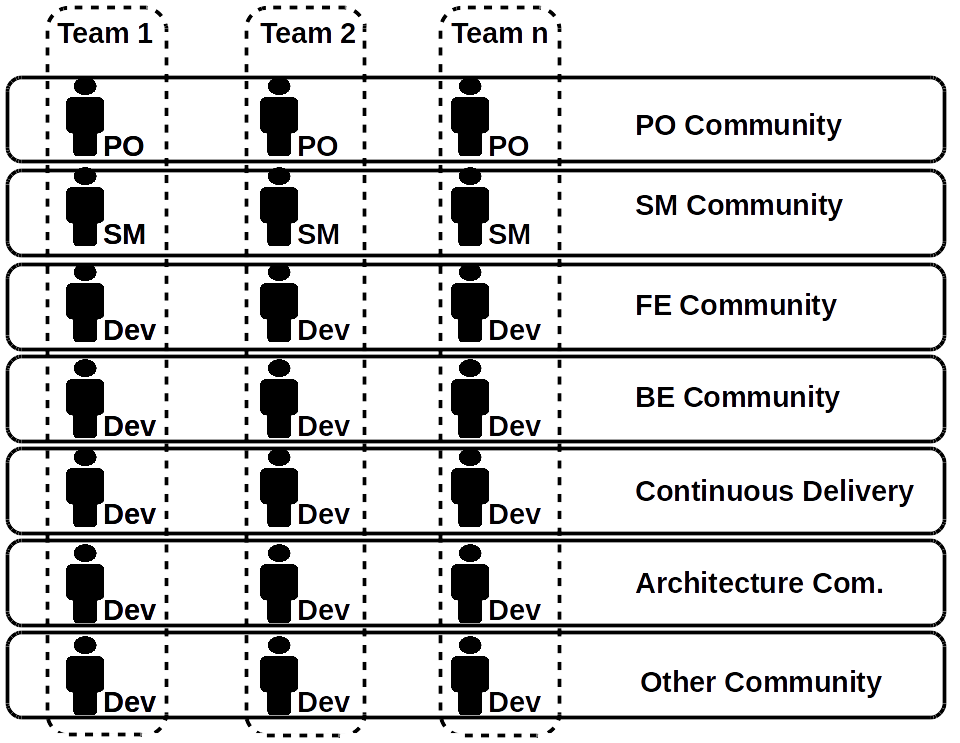
\includegraphics[width=0.60\textwidth]{Communities}
  \caption{Ejemplo de comunidades}
  \centering
  \label{fig:Communities} %\ref{fig:Communities}
\end{figure}


\subsection{Integración UX}

Un desafío a la hora de hacer Scrum es incorporar UX en el desarrollo incremental por sprints. Se pueden adoptar, entre otras, dos estrategias principales: desarrollo UX distribuido y gobernado; o desarrollo UX centralizado (equipo externo).

\subsubsection{Desarrollo UX Distribuido y Gobernado}

Una estrategia es tener UXer, como miembros de equipo Scrum, distribuidos en cada equipo. Esto permite empoderamiento y velocidad, pero puede generar una UX poco unificada o con poca “integridad conceptual”. Para resolver este problema de unificación se puede acudir a la estandarización UX. La misma podría ser generada y mantenida por los equipos o mediante un equipo externo responsabilizado de la integridad conceptual y experiencia unificada (equipo de estandarización UX transversal) y usar un sistema de versionado de estándares que sirve como otra herramienta de coordinación.

\subsubsection{Desarrollo UX Centralizado}

Otra estrategia es tener un equipo externo de UX que agrupe a todos los UXer y que provea, como un equipo de servicios, los diseños UX a los equipos de desarrollo. Sin embargo, es probable que el equipo central se convierta en un “cuello de botella” para los equipos de desarrollo y, además, pueda generar más “dependencias” que deben ser abordadas. Para mitigar estos problemas, un modelo híbrido a menudo puede ser aplicado, además de mecanismos de coordinación entre el equipo central y los equipos restantes.

\subsubsection{Mecanismo de coordinación de tarea UX en una historia}

En ambas propuestas es necesario coordinar e integrar el flujo de trabajo UX con el flujo de desarrollo Scrum. Esto sucede principalmente porque el flujo de trabajo UX no suele entrar dentro de un sprint corto (dos semanas) para que las historias puedan ser finalizadas. Lo que se puede hacer, es que el trabajo UX sea previo al sprint (adelantado al sprint) como parte de la etapa de refinamiento, o como etapa previa al compromiso de planning de sprint. La historia no se termina de refinar o no se compromete en un sprint, hasta que no se considera el trabajo UX lo suficientemente maduro como para que sea abordada para desarrollo. Una manera de hacer esta sincronización es agregando una cláusula de completitud de tarea UX al DoR de la historia. Y, además, asociando a las historias tareas UX que, a su vez, tengan DoR y DoD propios. De este modo, una tarea UX no se considera terminada, para que su historia asociada sea abordada en un sprint, si no cumple su “DoD UX”. Además, para trabajar a sprint adelantado hay que considerara que antes del sprint 1 debería hacerse un sprint 0 (sprint metáfora y/o inception).

\begin{figure}[h]
  \centering
  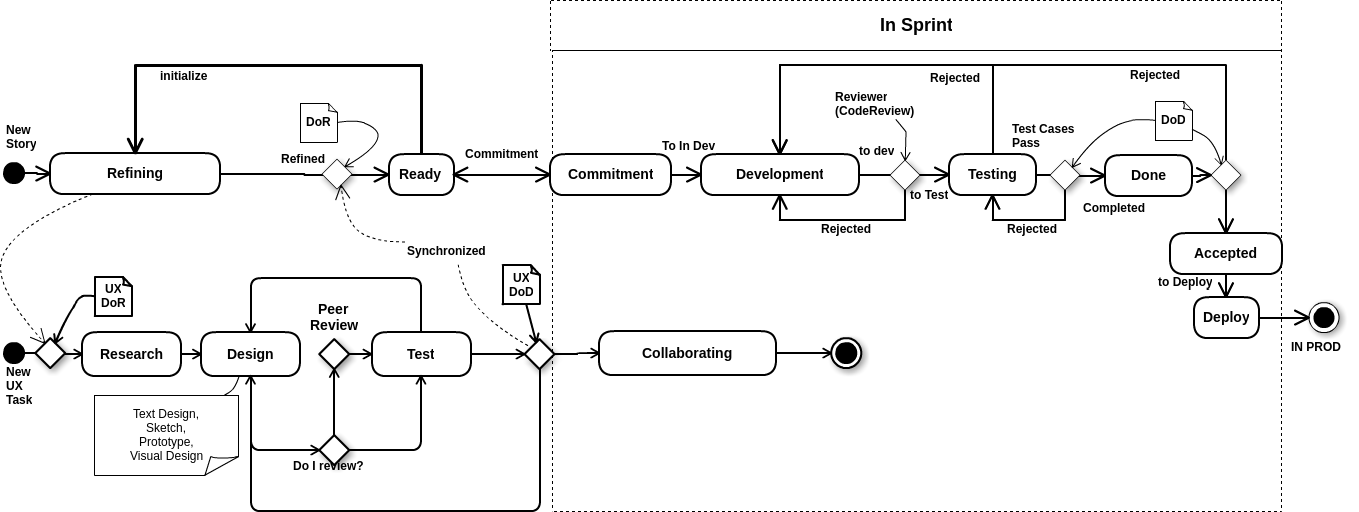
\includegraphics[width=1\textwidth]{UXtask-and-Story-in-Scrum}
  \caption{Ejemplo de coordinación entre flujos de tarea UX e historia}
  \centering
  \label{fig:UXtask-and-Story-in-Scrum} %\ref{fig:UXtask-and-Story-in-Scrum}
\end{figure}

\subsection{DevOps}

La integración a escala para que una Software Factory sea ágil y lleve adelante uno de sus principios, el Continuous Delivery, es lo que se denomina DevOps. DevOps es la integración de Ingeniería de Desarrollo de Software con la Ingeniería de Operaciones, que es todo el soporte IT y de plataforma para posibilitar que el proceso de desarrollo sea ágil, haciendo entregas frecuentes de calidad y logrando la colaboración entre el personal de desarrollo y el personal de operaciones a lo largo de todas las etapas del ciclo de vida de producción de software. DevOps es una parte central del agilismo en la entrega de software eficiente, por medio de la integración de equipos, metodologías ágiles, técnicas y stack tecnológico como una sola organización. El objetivo principal de DevOps es minimizar los cuellos de botella en el pipeline de entrega, haciéndolo más eficiente y ágil \footnote{\cite{DevOps-for-dummies-2015}}.

\begin{figure}[h]
  \centering
  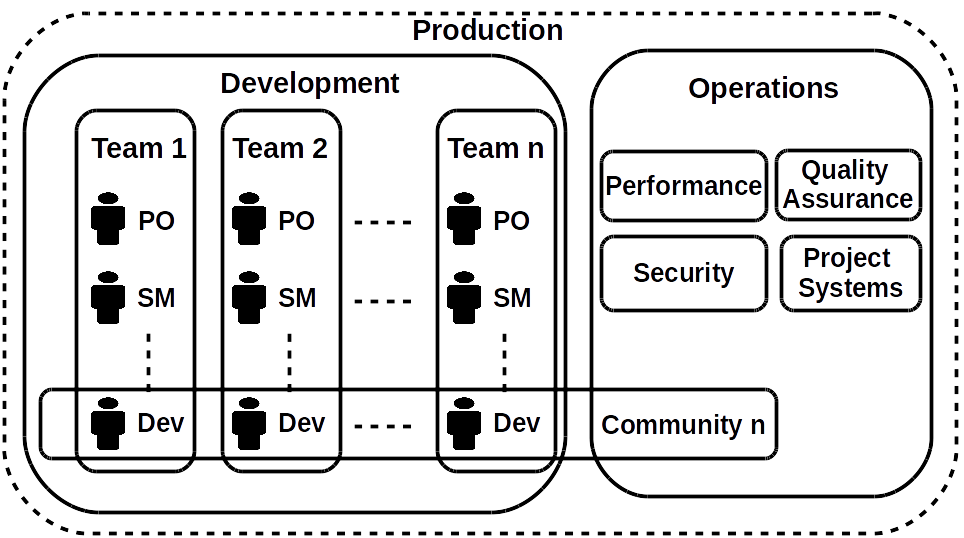
\includegraphics[width=0.80\textwidth]{DevOps}
  \caption{Ejemplo de integración de equpos en DevOps}
  \centering
  \label{fig:DevOps} %\ref{fig:DevOps}
\end{figure}

Una manera de integrar Operaciones con Desarrollo es mediante el uso de herramientas compartidas, misma cultura, comunidades en común, procesos ágiles compartidos, comunicación estandarizada, etcétera. Algo crucial en una organización madura es la automatización máxima en procesos de Continuous Integration y Continuous Delivery.

En cuanto a Scrum, el área de operaciones no necesita implementar Scrum, pero sí puede llevar en práctica sus valores, ser ágil (con Lean, Kanban, DAD, etc.) y tener en cuenta los ciclos Scrum de los equipos de desarrollo. DevOps es sólo un paso importante para unirse a la cultura general de la colaboración ágil y que debe involucrar a todas las disciplinas en una organización. 


\section{Modelos de escalamiento}

Existen diversos modelos, marcos y frameworks para escalamiento como lo son el modelo Spotify, SAFe, LeSS, Nexus, DAD, Lean Management, Agile Portfolio Management (APM), Recipes for Agile Governance in the Enterprise (RAGE) y otros. A continuación una breve reseña de algunos de ellos.

\subsection{Spotify}

Spotify es un caso de estudio que demuestra que puede ser aplicado más allá de pequeñas empresas o startup, sino en empresas más grandes (Spotify constaba en 2014 de aproximadamente de 250 personas en tres países). Por este motivo es un modelo de referencia. El modelo de Spotify consta de equipos escuadrones (squad), equivalentes a Equipos Scrum, con un PO y un SM llamado también Team Facilitator (Coach del equipo). Los escuadrones relacionados se agrupan en tribus (tribe) de no más de 100 personas, conformando un área de producto (como por ejemplo un tipo de producto) o área funcional (como por ejemplo infraestructura). La tribu tiene un líder de tribu (Tribe lead) quien se encarga de asegurar un alto rendimiento de la tribu, dar soporte a los líderes de los capítulos, facilitar y entrenar a los SM y construir liderazgo dentro de la tribu. 

\begin{figure}[h]
  \centering
  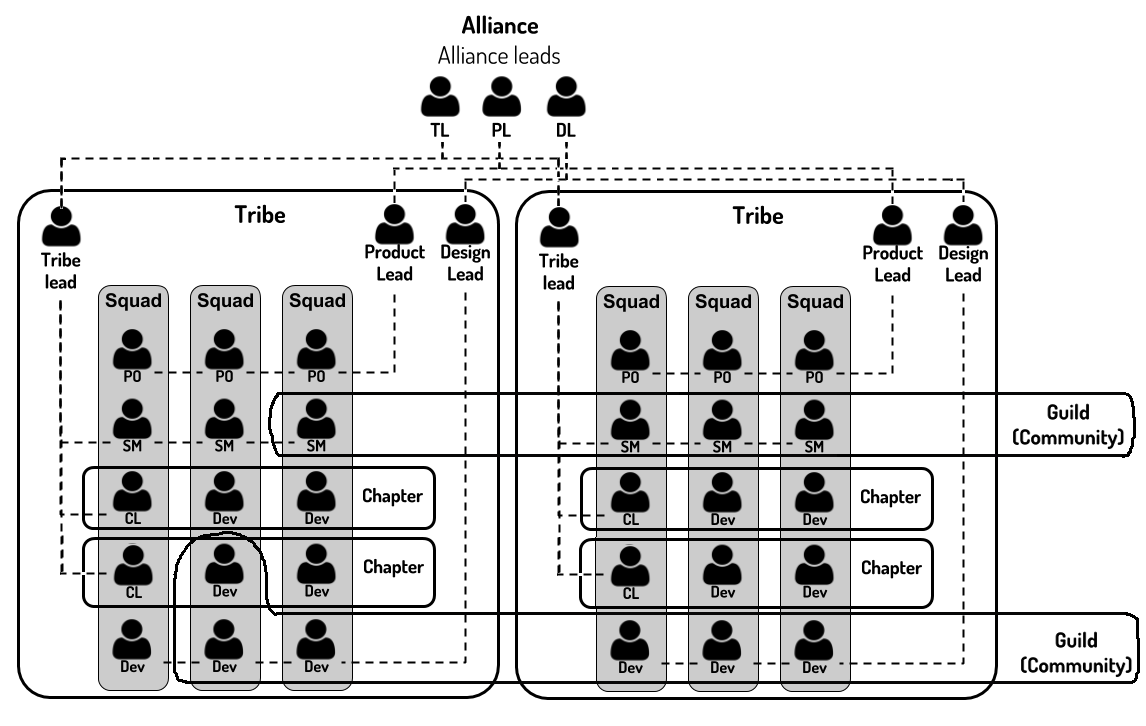
\includegraphics[width=0.99\textwidth]{Spotify_organizational_model}
  \caption{Modelo organizacional Spotify}
  \centering
  \label{fig:Spotify_organizational_model} %\ref{fig:Spotify_organizational_model}
\end{figure}

La tribu también tiene un líder de producto (PL) y uno de diseño (DL). Dentro de cada tribu hay capítulos (Chapter) y cada uno engloba un área funcional técnica de ingeniería, agrupando a los miembros de diferentes escuadrones con habilidades similares y que trabajan dentro del mismo área de competencia (por ejemplo el capítulo QA, BE, FE, etc.). Cada capítulo tiene un líder del capítulo ("Chapter lead" o CL) quien se encarga del desarrollo profesional, la cultura de la ingeniería, el apoyo del escuadrón y en asegurar la contratación de las personas adecuadas. Los líderes de capítulo suelen ser desarrolladores a tiempo parcial, por lo general se sientan en uno de los escuadrones de la tribu. 
Las diferentes tribus se pueden relacionar de diferentes maneras. Dos de ellas son la alianza (Alliance) y las comunidades (Guild). Una comunidad es una "comunidad de interés" (explicadas anteriormente). Los capítulos siempre son locales para una tribu, mientras que una comunidad generalmente es transversal a varias tribus. Cada comunidad puede tener un "coordinador de comunidad" y su alcance es más flexible. Y por último, la alianza une a diferentes comunidades por cohesión funcional de producto y tiene tres líderes serviciales (TL, PL y DL) quienes facilitan el trabajo de los líderes de las tribus unidas y el funcionamiento de las tribus, en general.

\subsection{SAFe}

El framework Scaled Agile Framework o SAFe consiste en una base de conocimientos de patrones integrados modulares, por niveles organizativos, destinados al desarrollo Lean-Agile a escala empresarial. Scrum se integra en SAFe en el primer nivel inferior organizativo, el nivel de equipo. A este nivel le siguen los niveles de programa, flujo de valor y portafolio. SAFe propone elementos opcionales de integración, un nuevo rol llamado Product Manager quien dirige a los POs de los equipos, otro nuevo rol llamado Release Train Engineer quien coordina a los SMs, la coordinación de backlogs por medio de un Backlog a nivel programa y la coordinación entre equipos por medio de eventos conjuntos y refinamientos, eventos trimestrales, System Team, Scrum of Scrums, Team Backlog y Team PO. SAFe propone que los equipos deben tener sus iteraciones sincronizadas y a tiempos periódicos deben tener una iteración de integración y planificación de todos los equipos o productos  (se planifican trenes de releases). Para más información hay que remitirse a la guía y definición de prácticas dada por el sitio web de SAFe.

\subsection{LeSS}

Por otro lado tenemos al framework Large-Scale Scrum o LeSS que  es un marco de desarrollo de productos que extiende Scrum con reglas de escalado y directrices sin perder los propósitos originales de Scrum. LeSS tiene un conjunto de principios alineados a Scrum y sumado el pensamiento sistémico. Además tiene alrededor de 28 reglas disponibles en 3 libros y propone diferentes mecanismos de coordinación como eventos conjuntos y refinamiento, CoP, SoS, Integración de código, feature teams y Area Product Owner. LeSS también propone subdivisiones de la organización por áreas de valor o Customer Value. Para más información hay que buscar en la guía del sitio web “less.works” y en diferentes libros que tratan el tema, como por ejemplo: Large-Scale Scrum, More with LeSS de Craig Larman y Bas Vodde.

\subsection{Modelo Nexus}

Nexus es un marco de trabajo para desarrollar y mantener iniciativas a escala de desarrollo de productos y software basado en Scrum. Fue creado por Ken Schwaber y Scrum.org. Es un exoesqueleto cuyo corazón es un conjunto de Equipos Scrum combinados para crear un Incremento Integrado, usando una única Lista de Producto Backlog, manteniendo "Listas de Pendientes" por Sprint y apoyados por un "Equipo de Integración Nexus" quien brinda soporte para asegurar que se produzca un Incremento Integrado. Para más información basta leer la "Guía Nexus" publicada en Scrum.org.

\subsection{DAD}

El marco de decisiones de procesos “Disciplined Agile Delivery” o DAD, brinda una orientación ligera para ayudar a las organizaciones a escalar agilidad y buscar optimizar sus procesos de tecnología de la información (IT) de una manera sensible al contexto ágil y DevOps. Para ello, muestra cómo las diversas actividades, como la entrega de soluciones, las operaciones, la arquitectura empresarial, la gestión de cartera y otros equipos y áreas trabajan juntas. Las reglas implicadas en este marco hacen que la empresa busque ser consciente y escalable. La referencia primaria para DAD es el libro “Disciplined Agile Delivery: A Practitioner's Guide to Agile Software Delivery in the Enterprise”,  escrito por Scott Ambler y Mark Lines.\newline
\newline

Si bien estos modelos tiene distintos grados de aceptación y éxito en muchas organizaciones, no se deben tomar como ley en piedra aplicándolos en cualquier contexto u organización. No se deberían implementar como recetas a seguir o soluciones ideales a implantar. Para aplicarlos en una organización deben ser evaluados y, en caso de aplicar alguna de sus pautas, ajustados según contexto y necesidades. Se recomienda aplicar también el pensamiento sistémico, ingeniería de sistemas y perspectivas de otras disciplinas.

\section{Equipo de mejora continua}

Como se ha visto, el escalamiento no es tarea simple y no existe una solución universal. Se puede dejar que los cambios organizacionales emerjan de abajo hacia arriba (desde los equipos, comunidades o individuos), sean dirigidos por un ente director (coaches, consultoras o un líder transformacional) o algo mixto. Hay frameworks que recomiendan que, cuando se desea llevar a cabo transformaciones organizacionales hacia la agilidad, se constituya un equipo de expertos ágiles llamado centro de excelencia, centro de transformación digital, centro de soporte ágil o equipo transversal de mejora continua \footnote{ScrumStudy recomienda un Scrum Guidance Body y DAD recominda un equipo de excelencia CoE.}. Este equipo se encargaría de hacer coaching a equipos y a otros roles, proponer iniciativas de mejoras organizacionales y apoyar la transformación cultural. El equipo puede estar formado por Coaches Ágiles Empresariales, gerentes ágiles, ingenieros de sistemas, ingenieros de operaciones, capital humano, etc. Los miembros deben ser capaces de trabajar en cualquier nivel de la organización, teniendo una visión multidisciplinaria, global y perspectiva sistémica.
